\chapter{Method}

\section{Data}

The data is collected during a 4,5 month pilot study which includes 20 patients.
All patients are at least 18 years old and have been injecting insulin at least 1 year prior to the study.
Each patient are equipped with a CGM sensor for the entirety of the study.
For each patient, the CGM sensor measures the blood glucose concentration (BGC) at intervals of 1-5 minutes.
The (time, BGC) tuples constitutes the structure of each patient's data set.
Additionally, other events such as meals and exercise are logged manually by patients.
A summary of collected data points are presented in Table \ref{table:data_description}.

\medskip
\begin{table}[ht!]
\begin{center}
  \begin{tabular}{lll}
  \textbf{Notation} &
  \textbf{Field} &
  \textbf{Format} \\
  \hline
  $P$ &
  Patient &
  Integer \\
  $t$ &
  Time &
  Date \\
  $t_{BG}$ &
  Glucose value at $t$ &
  Float \\
  $t_{ACT}$ &
  Physical activity at $t$ &
  Integer \\
  $t_{INS}$ &
  Injected insulin at $t$ &
  Float \\
  $t_{IMG}$ &
  Food image at $t$ &
  Float \\
  $t_{EVENT}$ &
  Manually reported by patient at $t$ &
  Text \\
  \hline
  \end{tabular}
  \caption[]
  {\small The data for each patient include continuous measurements at time steps $t$ of intervals between 1-5 minutes. Each measurement at $t$ \textit{always} include BG value and \textit{may} contain other field presented in the table.}
  \label{table:data_description}
\end{center}
\end{table}


\section{Implementation}

The objective of the proposed system is to analyze the data for a closed time interval, identify events and classify them accordingly with respect to their influence over future measurements.
The analysis is not performed in real time, all data is available immediately to the algorithms.
The proposed steps of implementation can be overviewed in Figure \ref{fig:flowchart}.
Each step is described in more detail in its corresponding section below.

\begin{figure}[ht!]
  \centering
  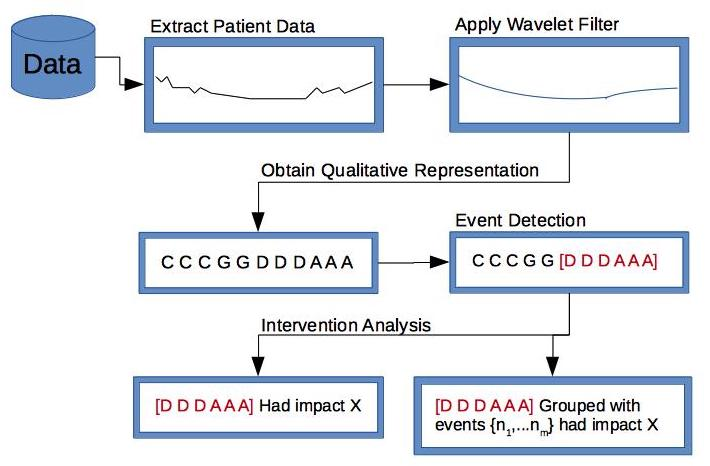
\includegraphics[width=0.8\textwidth]{images/flowchart.jpg}
  \caption[]
  {\small Schematics of implementation.}
  \label{fig:flowchart}
\end{figure}


\subsection{Wavelet Filter}

Studies have shown data from CGM sensors is subject to distortion.
This is caused by diffusion processes and by time-varying systematic under/overestimations due to calibrations and sensor drifts \parencite{facchinetti2014modeling}.
Noise can trigger false positives in event detection because abrupt fluctuations overrides the true underlying derivatives of the curve \parencite{Facchinetti2016}.
Wavelet filters have been used repeatedly with CGM data and proved successful in reducing noise while retaining events such as spikes \parencite{Mag2016}, \parencite{Facchinetti2016}, \parencite{samadi2017}.
Figure \ref{fig:wavelet_example} displays an example of wavelet filtering applied to CGM data.

\begin{figure}[ht!]
  \centering
  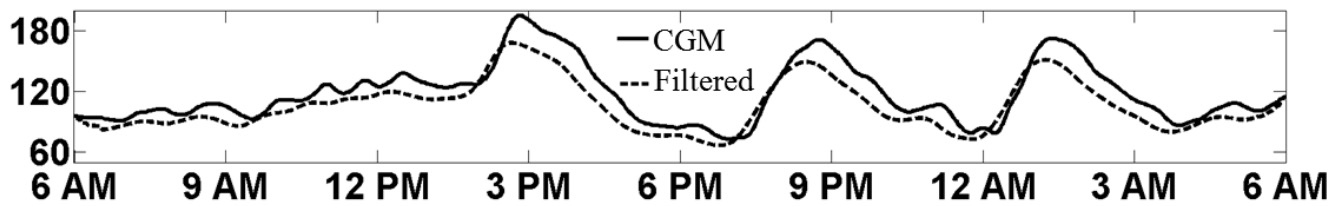
\includegraphics[width=0.6\textwidth]{images/wavelet_example.jpg}
  \caption[]
  {\small Wavelet filter applied on CGM data. Vertical axis represents glocose concentration [mg/dl]. Image courtesy of \textcite{samadi2017}.}
  \label{fig:wavelet_example}
\end{figure}


\subsection{Qualitative Representation}

To identify events in the de-noised CGM data, feature extraction is used.
Feature extraction can be achieved by either a qualitative or quantitative method.
The qualitative method offer benefits such as more transparent reasoning and ability to provide explanations for for the solutions it provides \parencite{Ven2003}.

In qualitative representation by triangular shapes, a CGM data segment can take seven shape variables.
Figure \ref{fig:shapes} shows the different shapes.
Each is a unique combination of the first and second order derivatives on the curve of the current segment.
The derivates can be read from segment of adjacent points, allowing the CGM data series to be presented as a sequence of shapes describing fluctuations in BGC.

\begin{figure}[ht!]
  \centering
  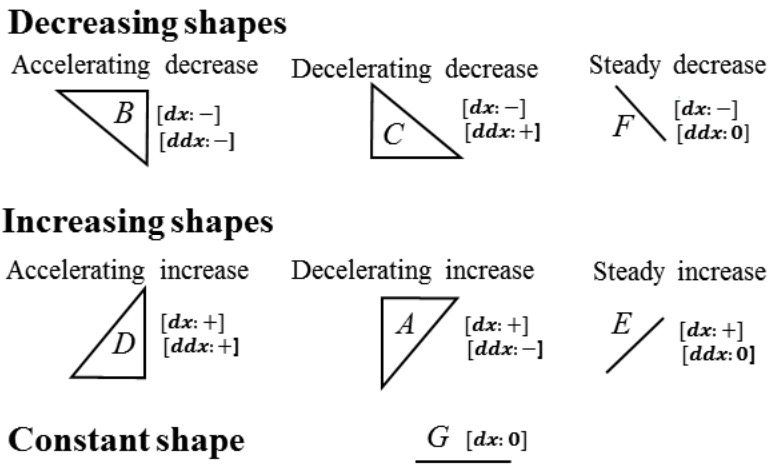
\includegraphics[width=0.6\textwidth]{images/shapes.jpg}
  \caption[]
  {\small Scheme of the qualitative variables A-G. Image courtesy of \textcite{samadi2017}.}
  \label{fig:shapes}
\end{figure}


\subsection{Event Detection}

With the qualitative representation, event detection can be performed by analyzing the sequence of shapes.
In figure \ref{fig:curve2shape} an event could be triggered by identifying a continuously accelerating increase (for example the four sequential D's from time-step 12).

\begin{figure}[ht!]
  \centering
  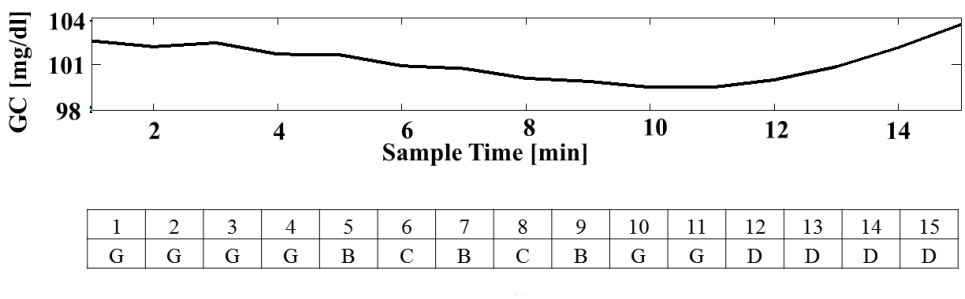
\includegraphics[width=0.8\textwidth]{images/curve2shape.jpg}
  \caption[]
  {\small Shape sequence representation if CGM curve. Image courtesy of \textcite{samadi2017}.}
  \label{fig:curve2shape}
\end{figure}


Given a sequence of observations (i.e. shapes) with some underlying state (i.e. eating, sleeping, exercising) a hidden Markov model can provide an estimate of what state a current time step most probably corresponds to.
The Markov approach includes two steps:

\textbf{The evaluation problem}: Calculating probability distribution by training a model on sequences with labeled states.

\textbf{The decoding problem}: Determining the hidden states by observing a unlabelled sequence and finding the optimal state sequence associated with the given observation sequence \parencite{rabiner1989}.

\subsection{Intervention Analysis}

Intervention analysis provides a tool to asses how much a given event has changes the series (if at all) \parencite{box2015time}.
The analysis is able to detect 4 patterns:

\begin{enumerate}
  \item Permanent constant change to the mean level.
  \item Brief constant change to the mean level.
  \item Gradual increase or decrease to a new mean level.
  \item Initial change followed by gradual return to previous mean level.
\end{enumerate}

The mean level in our case is the mean BGC.
Intervention analysis compare the mean average before the event and its progression afterwards.
The characteristics of the progression curve defines which of the four patterns an event has triggered.
Because changes in mean BG concentration are subtle and changes takes place over a longer timespan, an alternative to the approach is suggested.

An event by itself may not cause a observable change in the mean average but combined events might.
The intervention analysis is also evaluated on sets of adjacent events.
The output can hint on when the aggregated data implies a positive development of the mean.
In other words, the analysis can suggest when combined activities by a patient results in a change of his or her long term HbA1c value.

\section{Evaluation}

The method is evaluated in two steps:

\textbf{Detection of events}: For each patient, a 80/20\% data split is made into training and test data respectively.
The training data is utilized to solve the Markov evaluation problem and find model parameters.
The labels are removed from the test data the events are produced from the Markov decoding step of the algorithm.
A comparison of the removed (true) labels and the proposed ones are made and accuracy and precision measurements serves the basis of this evaluation.

\textbf{Intervention analysis}: Given that the algorithm has produced a set of events with suggested interventions.
A clinician is presented the same data and suggested events.
The clinician performs a independent assessment of the probable intervention caused by these events.
The algorithmic output is then compared to the clinicians and an accuracy and precision score is studied to evaluate the performance of the intervention analysis.
